\chapter{Lab Techniques II: Synthesis and Analysis in Practice}\label{ch:b2:lab-techniques-2}

A Grignard reaction fails on a Monday morning: the flask had been rinsed but not dried, and the few
drops of water left in it destroyed the reagent as it formed. Run again in glassware dried in an oven,
under nitrogen, with the halide added drop by drop into a stirred, cooled flask, the same reaction
works. The chemistry did not change; the set-up did. This chapter is about the practice that turns a
reaction on paper into a product in a vial: controlling the reaction, keeping air and water out,
working it up, purifying it and proving what was made.

\begin{omfigure}
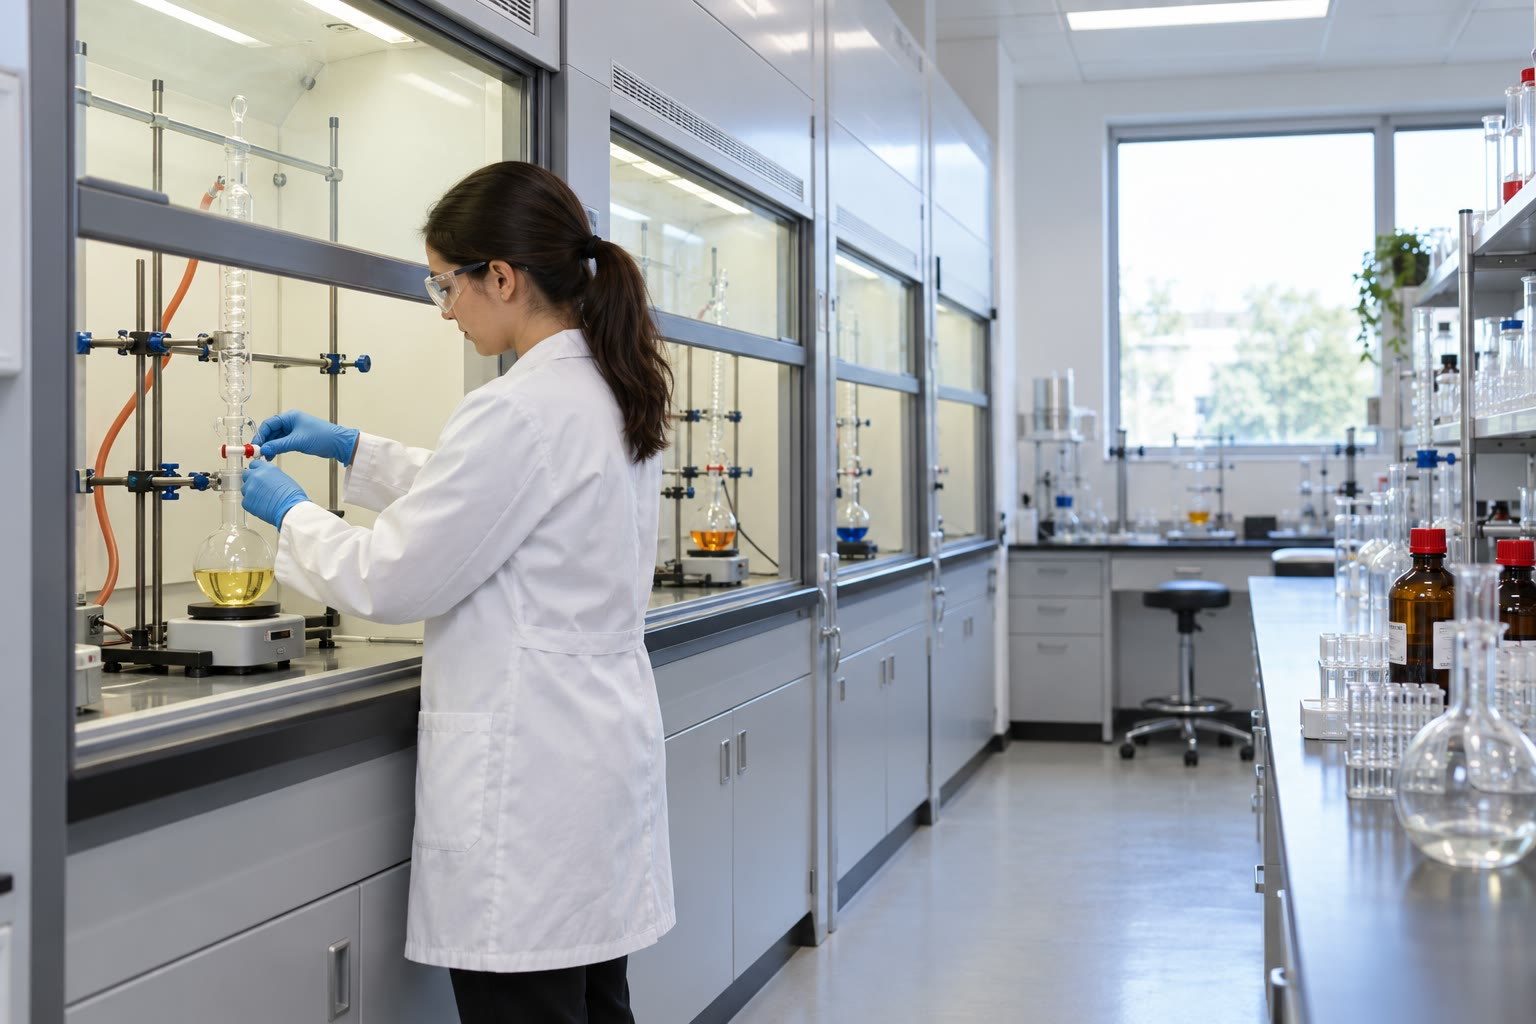
\includegraphics[width=0.56\linewidth]{images/book3/ai/b2-35-synthesis-lab.jpg}

{\small An organic synthesis laboratory: reactions run in fume hoods, flasks clamped on stands
(illustration).}
\end{omfigure}

\begin{recall}
The Year 1 volume: hazards and GHS labels, extraction, recrystallisation, distillation, thin-layer
\omterm{def:b2:chromatography:principle}{chromatography} and $R_f$, melting point, Grignard reagents. \Cref{ch:b2:reaction-enthalpy}: \omterm{def:b2:reaction-enthalpy:reaction-quantity}{reaction
enthalpy} and \omterm{def:b2:continuous-reactors:adiabatic-rise}{adiabatic temperature rise}. \Cref{ch:b2:chromatography},
\cref{ch:b2:structure-determination} and \cref{ch:b2:measurement-statistics}: analysis.
\end{recall}

\section{Running a reaction under control}

A reaction in a flask releases its heat where it happens. The chemist controls temperature with a bath
(ice and water, ice and salt, dry ice and acetone for the lowest temperatures), with the reflux of a
boiling solvent, which caps the temperature at its boiling point while the condenser returns the
vapour, and by the rate at which a reagent is added. An internal thermometer, in the liquid rather than
in the bath, measures what matters.

\begin{proposition}[Accumulation]\label{prop:b2:lab-techniques-2:accumulation}
If a reagent is added faster than it reacts, the unreacted amount $n_{\mathrm{acc}}$ accumulates. Should
it then react all at once, with no cooling, the temperature of the mixture of heat capacity $C$ rises by
\begin{equation*}
\Delta T_{\mathrm{ad}} = \frac{n_{\mathrm{acc}}\,|\Delta_rH|}{C}.
\end{equation*}
\end{proposition}

\begin{proof}
The reaction of $n_{\mathrm{acc}}$ releases $n_{\mathrm{acc}}|\Delta_rH|$ at constant pressure
(\cref{ch:b2:reaction-enthalpy}); without heat exchange, all of it warms the mixture, as in the
\omterm{def:b2:reaction-enthalpy:flame-temperature}{adiabatic flame temperature} (\cref{def:b2:reaction-enthalpy:flame-temperature}): $C\Delta T =
n_{\mathrm{acc}}|\Delta_rH|$.
\end{proof}

The danger is greatest when a reaction is slow to start, as Grignard formations often are: halide added
before initiation piles up, and when the reaction finally starts it runs away. The rule is to add a small
portion, see the reaction start (warming, cloudiness, gentle reflux), and only then add the rest at the
rate the cooling can follow.

\section{Dry conditions and inert atmosphere}

\begin{definition}[Inert atmosphere]\label{def:b2:lab-techniques-2:inert}
A reaction is run under an \emph{inert atmosphere}\index{inert atmosphere} when the air in the apparatus
has been replaced by an unreactive gas, nitrogen or argon, kept at a slight overpressure so that air
cannot enter.
\end{definition}

Organometallic reagents, metal hydrides and many catalysts react with water and oxygen. Glassware is
dried in an oven and assembled warm, or flamed under a stream of gas; solvents are bought dry or dried
over a reagent that reacts with water; liquids are transferred with syringes through rubber septa.
The gas leaves through an oil bubbler, which shows the flow and stops air from flowing back. The
Schlenk line and the glovebox, for the most sensitive compounds, come in the Year 3 volume.

\begin{omfigure}
\begin{tikzpicture}[lab/.style={font=\scriptsize, align=center}]
\fill[omDef!10] (-1.7,-0.3) rectangle (1.7,1.0);
\draw[om glass] (-1.7,1.2) -- (-1.7,-0.3) -- (1.7,-0.3) -- (1.7,1.2);
\foreach \x/\y in {-1.5/0.0,-1.45/0.55,1.3/0.05,1.3/0.6,-1.25/0.3,1.05/-0.15}{
  \draw[omDef!50, fill=white] (\x,\y) rectangle ++(0.18,0.18);}
\pic (f) at (0,0) {threeneck={0.35}{omThm!25}};
\pic[rotate=25] (d) at (f-l) {dropfunnel={0.5}{omMeth!20}};
\pic (c) at (f-c) {condenser};
\pic[rotate=-25] (t) at (0.0,0.42) {thermometer};
\pic (b) at (3.6,3.6) {bubbler};
\draw[thick, black!60] (0,6.25) -- (0,6.75) -- (3.25,6.75) -- (b-in);
\coordinate (dtop) at ($(f-l)+(-1.52,3.26)$);
\draw[thick, black!60] (dtop) -- ++(0,0.35) -- ++(-0.9,0) node[left, lab] {N$_2$};
\node[lab, anchor=north] at (0,-0.4) {ice bath};
\node[lab, anchor=east] at (-1.9,2.6) {addition\\funnel};
\node[lab, anchor=west] at (0.55,5.0) {condenser};
\node[lab, anchor=west] at (1.75,2.6) {thermometer\\(internal)};
\node[lab, anchor=north] at (3.6,3.45) {bubbler (gas out)};
\end{tikzpicture}
\par\vspace{4pt}

{\small A reaction under nitrogen (schematic). Three-necked flask in an ice bath, with an internal
thermometer in the liquid; the reagent is added from a pressure-equalising funnel through which the
nitrogen enters; the gas leaves through the condenser and an oil bubbler.}
\end{omfigure}

\begin{method}[Setting up a dry reaction under nitrogen]\label{met:b2:lab-techniques-2:anhydrous}
\begin{enumerate}
  \item Dry the glassware in an oven and assemble it hot, greasing or sleeving the joints; fit a septum
        or the addition funnel, the condenser and the bubbler.
  \item Flush with nitrogen while it cools; keep a slow flow (a bubble every second or two) throughout.
  \item Add solids before flushing, dry solvents and liquid reagents by syringe or cannula through a
        septum.
  \item Cool or heat as planned; start the addition with a small portion and check that the reaction
        starts before going on.
\end{enumerate}
\end{method}

\section{Work-up}

\begin{definition}[Work-up]\label{def:b2:lab-techniques-2:work-up}
The \emph{work-up}\index{work-up} of a reaction is the sequence of operations, after the reaction, that
turns the reaction mixture into the crude product: quenching, extraction and washing, drying,
filtration and evaporation of the solvent.
\end{definition}

\begin{definition}[Acid--base extraction]\label{def:b2:lab-techniques-2:acid-base-extraction}
An \emph{acid--base extraction}\index{acid--base extraction} separates acidic, basic and neutral organic
compounds dissolved in an organic solvent by washing the solution with aqueous acids or bases, which
convert one class of compounds into ions that pass into the water.
\end{definition}

\begin{proposition}[Who goes where]\label{prop:b2:lab-techniques-2:acid-base-extraction}
Aqueous sodium hydrogencarbonate (pH 8.3) extracts a carboxylic acid ($\mathrm pK_a$ about 4) but not a
phenol ($\mathrm pK_a$ about 10), which needs sodium hydroxide; dilute hydrochloric acid extracts an
amine whose conjugate acid has a $\mathrm pK_a$ of 4.6 or more; neutral compounds stay in the organic
layer.
% ledger: ph:NaHCO3, pka:benzoic, pka:phenol, pka:anilinium
\end{proposition}

\begin{proof}
A species is mainly in its basic form when $\mathrm{pH} > \mathrm pK_a$, and in more than 99~\% when
$\mathrm{pH} > \mathrm pK_a + 2$. At pH 8.3, benzoic acid (4.2) is more than 99~\% benzoate, an ion
that stays in the water; phenol (9.99) is about 2~\% phenoxide ($10^{8.3 - 10.0}$) and stays essentially
in the organic layer, where the neutral form partitions. In sodium hydroxide (pH above 12) phenol is
converted to phenoxide. In dilute hydrochloric acid (pH about 1), aniline (anilinium 4.6) is more than
99~\% anilinium. Each ion, once in water, is recovered by bringing the pH back the other way, which
regenerates the neutral compound, then extracting it again.
\end{proof}

\begin{omfigure}
\begin{tikzpicture}[x=1cm, y=1cm, st/.style={draw=black!70, rounded corners=2pt, fill=white,
  font=\scriptsize, align=center, inner sep=3pt, text width=3.0cm}, ar/.style={->, thick, black!70}]
\node[st, fill=omDef!10] (m) at (0,0) {benzoic acid, phenol,\\aniline, naphthalene\\in ethoxyethane};
\node[st, fill=omThm!10] (a1) at (5.0,0) {aqueous: benzoate\\$\to$ HCl $\to$ benzoic acid};
\node[st] (o1) at (0,-1.6) {phenol, aniline,\\naphthalene};
\node[st, fill=omThm!10] (a2) at (5.0,-1.6) {aqueous: phenoxide\\$\to$ HCl $\to$ phenol};
\node[st] (o2) at (0,-3.2) {aniline, naphthalene};
\node[st, fill=omThm!10] (a3) at (5.0,-3.2) {aqueous: anilinium\\$\to$ NaOH $\to$ aniline};
\node[st, fill=omMeth!10] (o3) at (0,-4.8) {naphthalene\\(dry, evaporate)};
\draw[ar] (m) -- node[above, font=\tiny] {NaHCO$_3$ wash} (a1);
\draw[ar] (m) -- (o1); \draw[ar] (o1) -- node[above, font=\tiny] {NaOH wash} (a2);
\draw[ar] (o1) -- (o2); \draw[ar] (o2) -- node[above, font=\tiny] {HCl wash} (a3);
\draw[ar] (o2) -- (o3);
\pic at (8.6,-3.6) {sepfunnel={omDef!25}{omThm!20}};
\node[font=\scriptsize, align=center] at (8.6,-4.0) {separating funnel};
\end{tikzpicture}
\par\vspace{4pt}

{\small Acid--base separation of four compounds (\cref{prop:b2:lab-techniques-2:acid-base-extraction}).
The organic layer (left column) loses one class at each wash; each aqueous extract (right) gives back
its compound when the pH is reversed.}
\end{omfigure}

\begin{definition}[Drying agent]\label{def:b2:lab-techniques-2:drying-agent}
A \emph{drying agent}\index{drying agent} is an anhydrous salt, such as magnesium or sodium sulfate,
that binds the water dissolved in an organic solution as water of hydration and is then removed by
filtration.
\end{definition}

\begin{method}[From the reaction flask to the crude product]\label{met:b2:lab-techniques-2:work-up}
\begin{enumerate}
  \item Quench: destroy the remaining reactive reagents with a suitable aqueous solution, slowly and with
        cooling.
  \item Extract into an organic solvent; separate the layers (check which is which by adding a drop of
        water); extract the aqueous layer again.
  \item Wash the combined organic layers (acid, base, then brine, a saturated sodium chloride solution
        that removes most of the dissolved water).
  \item Dry with a \omterm{def:b2:lab-techniques-2:drying-agent}{drying agent} until some of it stays free-flowing; filter.
  \item Remove the solvent on a rotary evaporator under reduced pressure; weigh the crude product.
\end{enumerate}
\end{method}

\section{Purification}

\begin{definition}[Flash chromatography]\label{def:b2:lab-techniques-2:flash}
\emph{Flash chromatography}\index{flash chromatography} is preparative column \omterm{def:b2:chromatography:principle}{chromatography} on silica in
which the eluent is pushed through the column by a slight gas pressure, so that a separation of grams
of material takes minutes; the eluent is chosen from thin-layer \omterm{def:b2:chromatography:principle}{chromatography} on the same silica.
\end{definition}

\begin{proposition}[Column volumes]\label{prop:b2:lab-techniques-2:column-volumes}
A compound that runs at $R_f$ on a TLC plate leaves a column of the same silica and eluent after
about $1/R_f$ column volumes of eluent.
\end{proposition}

\begin{proof}[Argument]
On the plate the compound travels $R_f$ times as far as the solvent front: its average speed is $R_f$
times that of the eluent. On the column the same partition gives the same ratio of speeds, so the
compound needs $1/R_f$ times the volume of eluent that fills the column (the hold-up volume) to come
out; in the language of \cref{ch:b2:chromatography}, $R_f \approx 1/(1 + k)$. A compound at $R_f = 0.25$
comes out after about four column volumes, well separated from one at 0.5 (two volumes).
\end{proof}

\begin{omfigure}
\begin{tikzpicture}[lab/.style={font=\scriptsize, align=left, anchor=west}]
\pic (k) at (0,0) {chromcolumn={3.4}};
\node[lab] at (0.6,4.6) {eluent};
\node[lab] at (0.6,3.55) {sand};
\node[lab] at (0.6,2.2) {silica bed};
\foreach \i/\c in {0/white, 1/omThm!25, 2/omThm!25, 3/white, 4/omDef!25, 5/omDef!25, 6/white}{
  \pic at ({2.4+0.55*\i},-1.2) {testtube={0.45}{\c}};}
\node[font=\scriptsize] at (4.05,-1.6) {fractions 1 to 7};
\pic at (7.6,-1.2) {tlcplate};
\foreach \j/\x in {2/7.15,3/7.45,5/7.75,6/8.05}{\node[font=\tiny] at (\x,-1.38) {\j};}
\fill[omThm] (7.45,0.95) circle (0.06); \fill[omThm] (7.15,0.95) circle (0.06);
\fill[omDef] (8.05,-0.05) circle (0.06); \fill[omDef] (7.75,-0.05) circle (0.06);
\node[font=\scriptsize, align=center] at (7.6,2.15) {TLC of the\\fractions};
\end{tikzpicture}
\par\vspace{4pt}

{\small \omterm{def:b2:lab-techniques-2:flash}{Flash chromatography} (schematic). The crude product is loaded on top of the silica and eluted;
the eluate is collected in fractions; a TLC plate of the fractions shows where each compound came out
(here the fast, nonpolar compound in fractions 2--3, the slower one in 5--6), and the pure fractions are
combined.}
\end{omfigure}

\begin{method}[Running a flash column]\label{met:b2:lab-techniques-2:flash}
\begin{enumerate}
  \item Choose the eluent by TLC: the wanted compound at $R_f$ about 0.25--0.35, as far as possible from
        the impurities.
  \item Pack the silica (about 30 to 100 times the mass of crude product) as a slurry or dry; add a layer
        of sand.
  \item Load the crude product in the least volume of solvent (or adsorbed on a little silica).
  \item Elute under slight pressure; collect fractions; check them by TLC; combine the pure ones and
        evaporate.
\end{enumerate}
\end{method}

Liquids that decompose near their boiling point are distilled at reduced pressure, where they boil
lower.

\begin{definition}[Distillation under reduced pressure]\label{def:b2:lab-techniques-2:reduced-pressure}
A \emph{distillation under reduced pressure}\index{distillation under reduced pressure} is carried out
in an apparatus connected to a vacuum pump through a manometer, at a pressure where the liquid boils at a
temperature it can stand.
\end{definition}

\begin{proposition}[Boiling at reduced pressure]\label{prop:b2:lab-techniques-2:reduced-pressure}
With $T_b$ the boiling temperature at the reference pressure $p^\circ$ and $\Delta_{\mathrm{vap}}H$
treated as constant, the boiling temperature at pressure $p$ is given by
\begin{equation*}
\frac{1}{T} = \frac{1}{T_b} - \frac{R}{\Delta_{\mathrm{vap}}H}\ln\frac{p}{p^\circ}.
\end{equation*}
\end{proposition}

\begin{proof}
A liquid boils when its vapour pressure equals the pressure above it. The Clausius--Clapeyron relation
of physics, $\mathrm d\ln p/\mathrm dT = \Delta_{\mathrm{vap}}H/(RT^2)$ for an ideal vapour and a
negligible liquid volume, integrates between $(T_b, p^\circ)$ and $(T, p)$ to $\ln(p/p^\circ) =
-(\Delta_{\mathrm{vap}}H/R)(1/T - 1/T_b)$; rearranging gives the result.
\end{proof}

\begin{omfigure}
\begin{tikzpicture}
\begin{axis}[width=0.72\linewidth, height=5.2cm, xmode=log, xmin=5, xmax=1100, ymin=0, ymax=190,
  xlabel={pressure (\unit{mbar})}, ylabel={boiling temperature (\unit{\degreeCelsius})},
  label style={font=\small}, tick label style={font=\scriptsize}, grid=major, grid style={black!10},
  legend style={font=\scriptsize, at={(0.02,0.98)}, anchor=north west}, legend cell align=left]
\addplot[omDef, thick] table[x=p, y=bromobenzene] {figdata/out/bachelor-2-vacuum-boiling.dat};
\addplot[omThm, thick] table[x=p, y=benzaldehyde] {figdata/out/bachelor-2-vacuum-boiling.dat};
\addplot[only marks, mark=o, mark size=2pt, omDef] coordinates {(7,27.75)};
\addplot[only marks, mark=o, mark size=2pt, omThm] coordinates {(13,61.85)};
\legend{bromobenzene, benzaldehyde, measured}
\end{axis}
\end{tikzpicture}

{\small Boiling temperature against pressure (\cref{prop:b2:lab-techniques-2:reduced-pressure}) with
the enthalpies of vaporisation and boiling points of the NIST WebBook. The circles are measured boiling
points at 7 and \qty{13}{mbar}, not used in the curves: the simple equation is within a few kelvin.
Lowering the pressure from 1 bar to \qty{20}{mbar} lowers the boiling points by more than
\qty{100}{K}.}
% figdata: bachelor-2/vacuum-boiling.py
% ledger: tb:bromobenzene, dvap:bromobenzene, tbp:bromobenzene.7mbar, tb:benzaldehyde, dvap:benzaldehyde, tbp:benzaldehyde.13mbar
\end{omfigure}

\section{Purity and identity}

A product is identified by comparing its spectra and physical constants with those of the expected
compound (\cref{ch:b2:structure-determination}); its purity is measured separately, because a product
can be the right compound and still contain several per cent of something else.

\begin{method}[Reporting purity and yield]\label{met:b2:lab-techniques-2:purity}
\begin{enumerate}
  \item Check the melting range of a solid (sharp and close to the literature value for a pure
        compound) and its TLC (one spot in two eluents).
  \item Measure purity: area per cent in GC or HPLC (only an estimate unless \omterm{def:b2:chromatography:quantitative}{response factors} are known,
        \cref{ch:b2:chromatography}), or quantitative proton NMR, comparing an integral of the product
        with one of each impurity, or with a weighed \omterm{def:b2:chromatography:quantitative}{internal standard}.
  \item Convert to a mass fraction $w$ of product in the isolated material.
  \item Report the yield corrected for purity: $\rho = w\,m/(n_{\mathrm{lim}}M)$, where $m$ is the
        mass isolated, $n_{\mathrm{lim}}$ the amount of limiting reagent and $M$ the molar mass.
\end{enumerate}
\end{method}

For an optically active product, the specific rotation adds a check of its stereochemical purity;
enantiomeric excess and its measurement are treated in the Year 3 volume.

\begin{safety}{\ghs[5mm]{GHS02}\,\ghs[5mm]{GHS06}\,\ghs[5mm]{GHS07}\,\ghs[5mm]{GHS08}\,\ghs[5mm]{GHS09}}
Ethoxyethane and oxolane are extremely flammable and form explosive peroxides on storage; no flame in
the laboratory, test old bottles before distilling. Bromobenzene is flammable and toxic to aquatic
life; magnesium turnings are flammable. Vacuum glassware is checked for star cracks and shielded.
% ledger: ghs:ether, ghs:THF, ghs:bromobenzene, ghs:Mg, ghs:MgSO4
\end{safety}

\section{Exercises}

\begin{exercise}[$\star$]\label{exo:b2:lab-techniques-2:1}
Which bath would you use for a reaction run at about \qty{0}{\degreeCelsius}, at about
\qty{-15}{\degreeCelsius}, and at \qty{-78}{\degreeCelsius}?
\end{exercise}

\begin{exercise}[$\star$]\label{exo:b2:lab-techniques-2:2}
An extraction uses dichloromethane, denser than water. Which layer is organic? How do you check?
\end{exercise}

\begin{exercise}[$\star$]\label{exo:b2:lab-techniques-2:3}
How do you know that enough magnesium sulfate has been added to an ether solution?
\end{exercise}

\begin{exercise}[$\star$]\label{exo:b2:lab-techniques-2:4}
In 4\,:\,1 hexane--ethyl acetate a product has $R_f = 0.65$ and an impurity 0.75. What would you change
for a column, and in which direction?
\end{exercise}

\begin{exercise}[$\star\star$]\label{exo:b2:lab-techniques-2:5}
Give the order of the washes that separate benzoic acid, phenol, aniline and naphthalene from an ether
solution, justifying each with a $\mathrm pK_a$, and how each compound is recovered.
\end{exercise}

\begin{exercise}[$\star\star$]\label{exo:b2:lab-techniques-2:6}
Estimate the boiling temperatures of bromobenzene and benzaldehyde at \qty{20}{mbar}.
\end{exercise}

\begin{exercise}[$\star\star$]\label{exo:b2:lab-techniques-2:7}
During an addition, \qty{0.050}{mol} of a reagent has accumulated unreacted. With $\Delta_rH =
\qty{-200}{kJ/mol}$ and a heat capacity of \qty{400}{J/K} for the mixture (exercise data), what
temperature rise could follow?
\end{exercise}

\begin{exercise}[$\star\star$]\label{exo:b2:lab-techniques-2:8}
An HPLC trace shows the product at 96.0~\% of the total area. Why is that not yet a mass purity? A
proton spectrum of the same sample shows a product singlet (1H) of integral 1.00 and an impurity singlet
(3H) of integral 0.12; product \qty{200}{g/mol}, impurity \qty{100}{g/mol} (exercise data). Compute the
mass fraction of product.
\end{exercise}

\begin{exercise}[$\star\star$]\label{exo:b2:lab-techniques-2:9}
\qty{4.10}{g} of a product (\qty{164}{g/mol}) of purity 95.0~\% (mass) are obtained from \qty{0.0300}{mol}
of limiting reagent. Compute the yield, uncorrected and corrected.
\end{exercise}

\begin{exercise}[$\star\star\star$]\label{exo:b2:lab-techniques-2:10}
A Grignard reaction gave benzene and almost no alcohol after addition of the aldehyde. List the
possible causes and how each is avoided.
\end{exercise}

\begin{exercise}[$\star\star\star$]\label{exo:b2:lab-techniques-2:11}
On scale-up, \qty{1.00}{mol} of a halide reacts with $\Delta_rH = \qty{-270}{kJ/mol}$ in a reactor whose
cooling removes at most \qty{150}{W} (exercise data). What is the shortest safe addition time? What
happens if the addition is faster?
\end{exercise}

\begin{exercise}[$\star\star\star$]\label{exo:b2:lab-techniques-2:12}
A crude solid of \qty{13.0}{g} could be purified by recrystallisation (one step, 80~\% recovery, purity
99~\%) or by \omterm{def:b2:lab-techniques-2:flash}{flash chromatography} (95~\% recovery, purity 99.5~\%, \qty{1.5}{L} of solvent) (exercise
data). Compare the two routes.
\end{exercise}

\section{Problem: A Grignard Done Right}

\begin{problem}[{Weekend problem --- hazards and a dry set-up, a controlled addition and the
accumulation danger, the work-up, purification by flash chromatography and a purity-corrected yield}]
\label{pb:b2:lab-techniques-2:1}
Exercise data. Phenylmagnesium bromide is made from \qty{15.7}{g} of bromobenzene and \qty{2.67}{g} of
magnesium turnings in dry ethoxyethane, then \qty{9.55}{g} of benzaldehyde is added; \omterm{def:b2:lab-techniques-2:work-up}{work-up} with
aqueous ammonium chloride gives diphenylmethanol. Formation of the reagent: $\Delta_rH =
\qty{-270}{kJ/mol}$; heat capacity of the mixture \qty{170}{J/K}; start at \qty{20}{\degreeCelsius}. TLC
(9\,:\,1 hexane--ethyl acetate): biphenyl $R_f = 0.85$, diphenylmethanol 0.25. Isolated after the column:
\qty{12.50}{g}. Proton NMR of this material: the \ce{CH(OH)} singlet (1H) integrates 1.00, the \omterm{def:b2:huckel:aromatic}{aromatic}
region 10.90. Molar masses (\unit{g/mol}): bromobenzene 157.01, benzaldehyde 106.12, diphenylmethanol
184.24, biphenyl 154.21; Mg 24.305.
% ledger: ghs:ether, ghs:bromobenzene, ghs:Mg, ghs:benzaldehyde, ghs:NH4Cl, ghs:biphenyl, ghs:benzhydrol, tb:ether, aw:Mg, aw:C, aw:H, aw:Br, aw:O, nmr:biphenyl

\medskip
\noindent\textbf{Part I --- Hazards and set-up.}
\begin{enumerate}
  \item Give the main hazards of ethoxyethane, bromobenzene and magnesium.
  \item Write the reaction of phenylmagnesium bromide with water, and explain the oven-dried glassware.
  \item Why work under nitrogen?
  \item What does the bubbler show, and what does it prevent?
  \item Why is ethoxyethane a good solvent here?
  \item Compute the amounts of bromobenzene and magnesium. Which is in excess?
\end{enumerate}

\medskip
\noindent\textbf{Part II --- Controlled addition.}
\begin{enumerate}[resume]
  \item What heat does the complete formation of the reagent release?
  \item Why is the bromobenzene added drop by drop?
  \item The reaction is slow to start, and 20~\% of the bromobenzene is added before it does. What heat
        can then be released at once?
  \item Compute the \omterm{def:b2:continuous-reactors:adiabatic-rise}{adiabatic temperature rise}.
  \item Compare the final temperature with the boiling point of ethoxyethane. What happens?
  \item How should the addition be conducted?
\end{enumerate}

\medskip
\noindent\textbf{Part III --- Addition and \omterm{def:b2:lab-techniques-2:work-up}{work-up}.}
\begin{enumerate}[resume]
  \item Write the reaction with benzaldehyde and identify the limiting reagent.
  \item Why quench with ammonium chloride rather than a strong acid?
  \item Which layer is organic in the separating funnel?
  \item What is the brine wash for?
  \item How is the solution dried, and how is the solvent removed?
  \item Biphenyl is the main by-product. How does it form, and what favours it?
\end{enumerate}

\medskip
\noindent\textbf{Part IV --- Purification and purity.}
\begin{enumerate}[resume]
  \item Which compound leaves the column first?
  \item After how many column volumes does each come out?
  \item From the NMR integrals, compute the molar ratio of biphenyl to alcohol in the isolated
        material.
  \item Compute the mass fraction of diphenylmethanol.
  \item Compute the mass of pure diphenylmethanol.
  \item Compute the theoretical mass.
  \item Compute the yield without correction for purity.
  \item State the yield corrected for purity.
\end{enumerate}
\end{problem}
